% Generated by code/scripts/report_figures.py at 2026-11-16T12:31:35Z; do not edit.
% Inputs: artifacts/cluster/runs/bench4-20261110T103706Z-1535991
\begin{figure}[t]
\centering
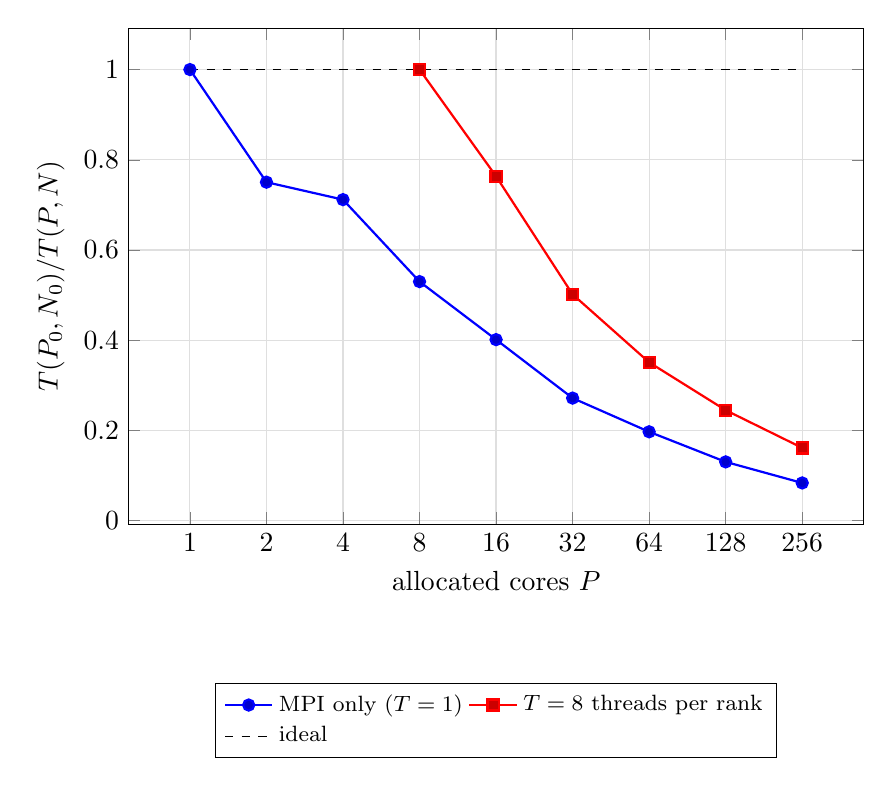
\begin{tikzpicture}
\begin{axis}[width=0.9\columnwidth, height=0.65\columnwidth, xlabel={allocated cores $P$}, ylabel={$T(P_0,N_0)/T(P,N)$}, xmode=log, log basis x=2, log ticks with fixed point, legend style={at={(0.5,-0.32)}, anchor=north, legend columns=2, font=\footnotesize}, legend cell align=left, grid=major, grid style={gray!25}]
\addplot+[mark=*, thick] coordinates {(1,1) (2,0.7504) (4,0.7117) (8,0.53) (16,0.4014) (32,0.2718) (64,0.1971) (128,0.1304) (256,0.08372)};
\addlegendentry{MPI only ($T=1$)}
\addplot+[mark=square*, thick] coordinates {(8,1) (16,0.7634) (32,0.5017) (64,0.351) (128,0.245) (256,0.1615)};
\addlegendentry{$T=8$ threads per rank}
\addplot[black, dashed] coordinates {(1,1) (256,1)};
\addlegendentry{ideal}
\end{axis}
\end{tikzpicture}
\caption{Weak-scaling efficiency. $T=1$: $P_0=1$, $N_0=50{,}000$, 50{,}000 particles per core; $T=8$: $P_0=8$, $N_0=400{,}000$, 50{,}000 particles per core. Constant particles per core is not constant work per core. Vanda job 1535991: 64 of 72 cores on each of four Platinum 8452Y nodes (CN-047, CN-061, CN-064, CN-065), 3 interleaved repetitions.}
\label{fig:b4-weak}
\end{figure}
